% ------------------
% -- Assignment 1 --
% -- Math 6904 -----

\documentclass[6pt,oneside]{article}

\usepackage{subcaption}
\usepackage{graphicx}
\usepackage{amsmath}
\usepackage{amsfonts}
\usepackage{adjustbox}
\usepackage{listings}
\usepackage{xcolor}
\usepackage{titlesec}
\usepackage{caption}
\usepackage{enumitem}
\usepackage{mathrsfs}
\usepackage{anyfontsize}
\usepackage[driver=pdftex]{geometry}
\usepackage{import}
\usepackage[ruled,vlined]{algorithm2e}
\usepackage{setspace}
\usepackage[utf8]{inputenc}
\usepackage{listingsutf8}
\usepackage[hidelinks]{hyperref}
\usepackage{cleveref}


\definecolor{codegreen}{rgb}{0,0.6,0}
\definecolor{codegray}{rgb}{0.5,0.5,0.5}
\definecolor{codepurple}{rgb}{0.58,0,0.82}
\definecolor{backcolour}{rgb}{0.95,0.95,0.92}
 
\lstdefinestyle{mystyle}{
    backgroundcolor=\color{backcolour},   
    commentstyle=\color{codegreen},
    keywordstyle=\color{magenta},
    numberstyle=\tiny\color{codegray},
    stringstyle=\color{codepurple},
    basicstyle=\fontsize{8}{10}\selectfont\ttfamily,
    breakatwhitespace=false,         
    breaklines=true,                 
    captionpos=t,                    
    keepspaces=true,                 
    numbers=left,                    
    numbersep=5pt,                  
    showspaces=false,                
    showstringspaces=false,
    showtabs=false,                  
    tabsize=2,
    literate={Δ}{$\Delta$}1 
    {₀}{{$_0$}}1 
    {α}{{$\alpha$}}1 
    {γ}{{$\gamma$}}1 
    {ρ}{{$\rho$}}1 
    {σ}{{$\sigma$}}1 
    {ₒ}{{$_o$}}1 
    {₁}{{$_1$}}1
    {ᵣ}{{$_r$}}1 
    {ₑ}{{$_e$}}1 
    {₂}{{$_2$}}1 
    {₃}{{$_3$}}1 
}
\lstset{style=mystyle}

\newtheorem{theorem}{Theorem}
\newtheorem{definition}{Definition}
\newtheorem{proof}{Proof}
 

\newcommand{\Real}{\mathbb{R}}
\newcommand{\Int}{\mathbb{Z}}
\newcommand{\Nat}{\mathbb{N}}
\newcommand{\Complex}{\mathbb{C}}
\newcommand{\vect}[1]{\boldsymbol{#1}}
\newcommand{\diag}[1]{\mathrm{diag}{#1}}
\newcommand{\Binom}[2]{\mathrm{Binomial}\left(#1,#2\right)}
\newcommand{\prob}[1]{\mathcal{P}\left(#1\right)}
\newcommand{\E}[1]{\mathcal{E}\left(#1\right)}
\newcommand{\set}{\leftarrow}
\renewcommand{\mod}[1]{\mathrm{mod}\;{#1}}

\renewcommand{\Re}[1]{\mathfrak{Re}\left\lbrace{#1}\right\rbrace}
\renewcommand{\Im}[1]{\mathfrak{Im}\left\lbrace{#1}\right\rbrace}

\makeatletter
\newcommand{\nosemic}{\renewcommand{\@endalgocfline}{\relax}}% Drop semi-colon ;
\newcommand{\dosemic}{\renewcommand{\@endalgocfline}{\algocf@endline}}% Reinstate semi-colon ;
\newcommand{\pushline}{\Indp}% Indent
\newcommand{\popline}{\Indm\dosemic}% Undent
\makeatother

\SetKwComment{Comment}{$\triangleright$\ }{}


\begin{document}

\section{1}

Write out a proof that $P$ is reversible with respect to $\mu$. Conclude that $\mu$ is an invariant
probability distribution for $P$.

\section{2}

Write out a proof that $P$ is irreducible, and that if $\mu$ isn't perfectly uniform, then $P$ is aperiodic.
\emph{[Hint: show that if $i\longrightarrow j$ under $Q$, then $i\longrightarrow j$ under $P$.
For aperiodicity, consider a site where a transition could be rejected.]}

Therefore, if you pick any state to start in and run the chain for a long time $n$ then the random
variable $X_n$ will be sampled from apximately the distribution $\mu$. Going further, $X_n,X_{n+1},
ldots, X_{n+m}$ will all have distributions approximately $\mu$. They won't be indepdendent, but
if $m$ is also large, then we can still show that

$$
\sum_i f(i)\mu_i \approx \frac{1}{m+1} \sum_{k=0}^m f(X_k).
$$

So expectations, with respect to the distribution $\mu$ can be worked out this way. This often works well in
practice, event though it is sometimes hard to get rigorous bounds on how large $n$ and $m$ must be for answers
to be reliable.

\vspace{10pt}

The Markov chain $P$ is irreducible if $i\longrightarrow j$ $\forall i,j\in\mathcal{S}$. First, we must show
that if $i\longrightarrow j$ under $Q$, then $i\longrightarrow j$ under $P$.

There are 2 cases to consider:

\begin{itemize}
    \item If $u_j \geq u_i$ as $i\longrightarrow j$, then we always accept the move; the probability is always 1.
\end{itemize}

\section{Results}

\begin{figure}[h]
    \center
    \caption{$l(i,j) \sim \mathrm{Gamma}(k=7.5)$}
    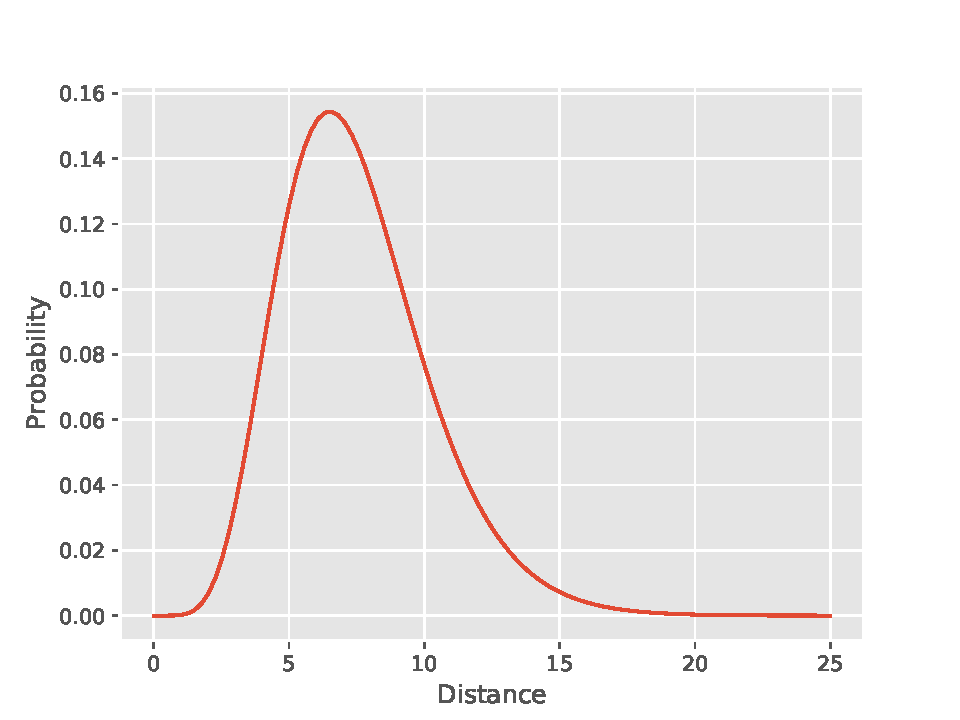
\includegraphics[scale=0.8]{../src/fig1.pdf}
\end{figure}


\begin{figure}[h]
    \center
    \caption{Several runs of Metropolis-Hastings algorithm $n=10^{6}$ and $m=10^{4}$}
    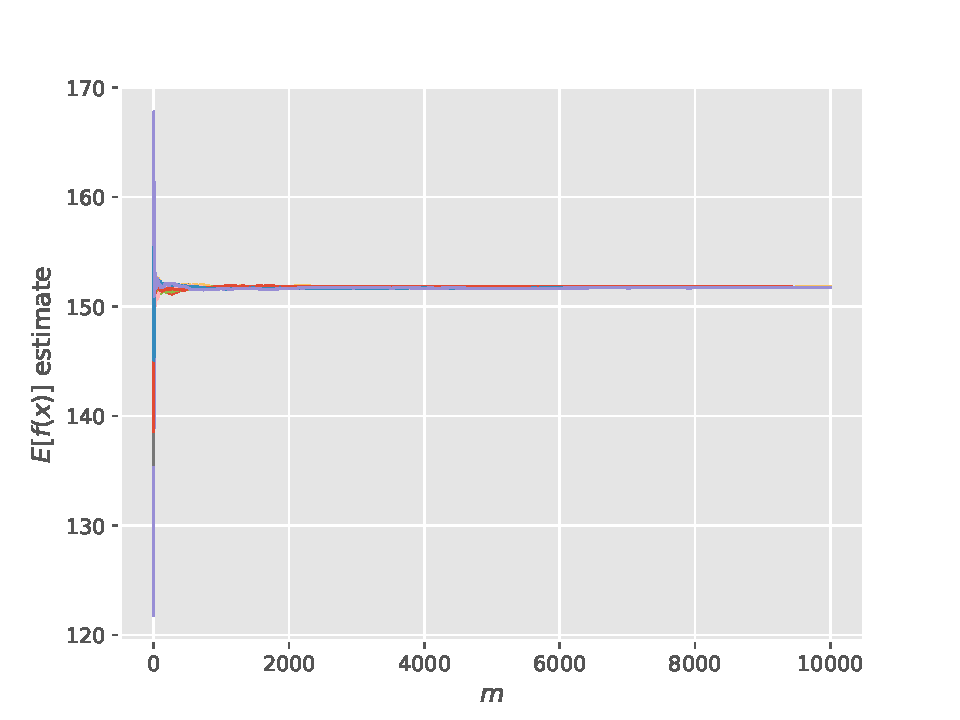
\includegraphics[scale=0.8]{../src/fig2.pdf}
    \footnotesize
    \vspace{10pt}

    \Cref{fig:12} shows the convergence of the MCMC. The burn-in phase is not depicted.
\end{figure}

\begin{table}[h]
    \center
    \caption{Results of 10 runs of Metropolis-Hastings algorithm}
    \label{fig:12}
    \begin{tabular}{rl}
        Run & $E\left[ f(x) \right]$ estimate \\
        \hline
        1 & 151.7582975592603 \\
        2 & 151.78521559558445 \\
        3 & 151.71995644022766 \\
        4 & 151.72257839116807 \\
        5 & 151.7989403512341 \\
        6 & 151.77048793781816 \\
        7 & 151.73434402770206 \\
        8 & 151.7712540561242 \\
        9 & 151.723880973142 \\
        10 & 151.7255789619957 \\
    \end{tabular}
\end{table}

\clearpage

\section*{Appendix}

\begin{table}[h]
    \center
    \caption{Distances between pairs of cities $(i,j)$ for $i,j \in \left\lbrace 0, 9\right\rbrace$ and $i\neq j$}
    \label{table:distances}
    \footnotesize
    \begin{tabular}{ccc|ccc|ccc|ccc|ccc}
        $i$ & $j$ & $ l(i, j)$ &
        $i$ & $j$ & $ l(i, j)$ &
        $i$ & $j$ & $ l(i, j)$ &
        $i$ & $j$ & $ l(i, j)$ &
        $i$ & $j$ & $ l(i, j)$
        \\
        \hline
0 & 1 & 11.26 & 2 & 11 & 13.25 & 8 & 10 & 4.95 & 11 & 4 & 7.32 & 16 & 18 & 6.79 \\
0 & 2 & 11.92 & 2 & 12 & 8.08 & 8 & 11 & 10.29 & 11 & 5 & 7.04 & 16 & 19 & 5.14 \\
0 & 3 & 6.02 & 2 & 13 & 15.34 & 8 & 12 & 7.86 & 11 & 6 & 6.13 & 17 & 2 & 4.03 \\
0 & 4 & 5.74 & 2 & 14 & 4.70 & 8 & 13 & 5.82 & 11 & 7 & 5.34 & 17 & 3 & 4.16 \\
0 & 5 & 8.05 & 2 & 15 & 13.81 & 8 & 14 & 3.23 & 11 & 12 & 14.47 & 17 & 4 & 6.58 \\
0 & 6 & 14.37 & 2 & 18 & 8.12 & 8 & 15 & 8.22 & 11 & 13 & 6.84 & 17 & 5 & 5.15 \\
0 & 7 & 9.05 & 2 & 19 & 4.63 & 8 & 16 & 6.86 & 11 & 14 & 13.87 & 17 & 6 & 7.10 \\
0 & 8 & 5.09 & 3 & 4 & 4.27 & 8 & 17 & 7.35 & 11 & 15 & 8.47 & 17 & 7 & 7.25 \\
0 & 9 & 10.81 & 3 & 5 & 9.03 & 8 & 18 & 4.50 & 12 & 5 & 6.70 & 17 & 10 & 6.54 \\
0 & 10 & 3.00 & 3 & 6 & 3.46 & 8 & 19 & 15.86 & 12 & 6 & 7.86 & 17 & 11 & 8.55 \\
0 & 11 & 7.43 & 3 & 7 & 3.77 & 9 & 2 & 11.78 & 12 & 7 & 6.49 & 17 & 12 & 3.17 \\
0 & 12 & 6.67 & 3 & 12 & 8.88 & 9 & 3 & 5.63 & 12 & 13 & 6.71 & 17 & 13 & 8.76 \\
0 & 13 & 3.04 & 3 & 13 & 9.89 & 9 & 4 & 6.60 & 12 & 14 & 11.08 & 17 & 14 & 9.74 \\
0 & 14 & 11.61 & 3 & 14 & 7.47 & 9 & 5 & 4.36 & 12 & 15 & 6.48 & 17 & 15 & 9.77 \\
0 & 15 & 6.37 & 3 & 15 & 9.96 & 9 & 6 & 8.22 & 13 & 5 & 9.27 & 17 & 18 & 6.96 \\
0 & 16 & 6.88 & 4 & 5 & 14.08 & 9 & 7 & 9.63 & 13 & 6 & 4.28 & 17 & 19 & 6.61 \\
0 & 17 & 7.25 & 4 & 6 & 4.28 & 9 & 10 & 7.84 & 13 & 7 & 13.30 & 18 & 3 & 3.94 \\
0 & 19 & 6.64 & 4 & 7 & 5.54 & 9 & 11 & 6.62 & 13 & 14 & 9.35 & 18 & 4 & 10.56 \\
1 & 2 & 6.89 & 4 & 12 & 6.72 & 9 & 12 & 6.46 & 13 & 15 & 5.58 & 18 & 5 & 13.23 \\
1 & 3 & 5.27 & 4 & 13 & 12.53 & 9 & 13 & 5.10 & 14 & 7 & 10.12 & 18 & 6 & 13.52 \\
1 & 4 & 5.11 & 4 & 14 & 9.28 & 9 & 14 & 6.23 & 14 & 15 & 5.13 & 18 & 7 & 10.42 \\
1 & 5 & 7.55 & 4 & 15 & 4.94 & 9 & 15 & 8.94 & 15 & 7 & 9.11 & 18 & 11 & 6.20 \\
1 & 6 & 6.03 & 5 & 6 & 4.72 & 9 & 18 & 10.98 & 16 & 1 & 7.09 & 18 & 12 & 8.71 \\
1 & 9 & 7.93 & 5 & 7 & 5.91 & 9 & 19 & 5.59 & 16 & 2 & 9.97 & 18 & 13 & 6.36 \\
1 & 11 & 11.22 & 5 & 14 & 8.21 & 10 & 3 & 7.85 & 16 & 3 & 6.82 & 18 & 14 & 5.02 \\
1 & 12 & 5.48 & 5 & 15 & 8.39 & 10 & 4 & 9.40 & 16 & 4 & 5.74 & 18 & 15 & 14.79 \\
1 & 13 & 8.99 & 6 & 7 & 5.08 & 10 & 5 & 7.12 & 16 & 5 & 6.00 & 18 & 19 & 5.46 \\
1 & 14 & 2.97 & 6 & 14 & 10.78 & 10 & 6 & 7.28 & 16 & 6 & 4.76 & 19 & 3 & 8.73 \\
1 & 15 & 5.40 & 6 & 15 & 5.37 & 10 & 7 & 6.48 & 16 & 7 & 9.43 & 19 & 4 & 6.78 \\
1 & 17 & 9.07 & 8 & 1 & 7.00 & 10 & 11 & 12.31 & 16 & 9 & 8.66 & 19 & 5 & 10.94 \\
1 & 18 & 5.72 & 8 & 2 & 6.02 & 10 & 12 & 4.34 & 16 & 10 & 4.08 & 19 & 6 & 8.01 \\
2 & 3 & 8.26 & 8 & 3 & 10.55 & 10 & 13 & 3.35 & 16 & 11 & 11.61 & 19 & 7 & 13.82 \\
2 & 4 & 4.77 & 8 & 4 & 5.51 & 10 & 14 & 2.68 & 16 & 12 & 9.64 & 19 & 11 & 4.46 \\
2 & 5 & 3.99 & 8 & 5 & 3.72 & 10 & 15 & 9.40 & 16 & 13 & 8.25 & 19 & 12 & 4.87 \\
2 & 6 & 6.67 & 8 & 6 & 6.77 & 10 & 18 & 4.39 & 16 & 14 & 10.74 & 19 & 13 & 7.57 \\
2 & 7 & 9.61 & 8 & 7 & 8.01 & 10 & 19 & 4.96 & 16 & 15 & 7.20 & 19 & 14 & 7.19 \\
2 & 10 & 7.26 & 8 & 9 & 12.26 & 11 & 3 & 8.05 & 16 & 17 & 7.78 & 19 & 15 & 4.11 \\

    \end{tabular}
\end{table}

\end{document}
